% Query-based summarization is a widely used benchmark for evaluating retrieval-augmented generation (RAG) systems~\cite{ram2023context, yu2023augmentation}. Recent work has also demonstrated the potential of GraphRAG for summarization tasks~\cite{edge2024local}. However, \citet{edge2024local} focus primarily on global summarization and rely on LLM-as-a-Judge~\cite{zheng2023judging} for evaluation. As shown in Section~\ref{sec:summ_analysis}, LLM-as-a-Judge introduces position bias in summarization evaluation, which can compromise result reliability. Despite the growing interest in GraphRAG, a systematic comparison between RAG and GraphRAG on general query-based summarization tasks across widely used datasets remains unexplored. To address this gap, we conduct a comprehensive evaluation in this section using standard benchmarks and evaluation metrics.





\begin{table*}[!htb]
\caption{The performance of query-based single document summarization task using Llama 3.1-8B.}
\label{tab:summ_single}
\vspace{-0.1in}
\resizebox{0.9\linewidth}{!}{
\begin{tabular}{l|cccccc|cccccc}
\toprule
\multirow{4}{*}{\textbf{Method}}      
& \multicolumn{6}{c|}{\textbf{SQuALITY}}                                                                           
& \multicolumn{6}{c}{\textbf{QMSum}} \\
\cmidrule{2-13}
& \multicolumn{3}{c}{\textbf{ROUGE-2}}                     
& \multicolumn{3}{c|}{\textbf{BERTScore}}                        
& \multicolumn{3}{c}{\textbf{ROUGE-2}}                    
& \multicolumn{3}{c}{\textbf{BERTScore}} \\ 
\cmidrule{2-13}
& P & R & F1 & P & R & F1 & P & R & F1 & P & R & F1 \\
\midrule
RAG                        
& 15.09 & 8.74 & 10.08 
& 74.54 & 81.00 & 77.62 
& \underline{21.50} & {3.80} & 6.32 
& {81.03} & 84.45 & {82.69} \\

RaptorRAG                  
& 14.88 & 8.42 & 9.81 
& 74.55 & 81.20 & 77.71 
& 20.38 & \textbf{4.17} & \textbf{6.68} 
& \textbf{81.64} & \underline{84.57} & \textbf{83.07} \\

KG-GraphRAG (Triplets only) 
& 11.99 & 6.16 & 7.41 
& 82.46 & 84.30 & 83.17 
& 13.71 & 2.55 & 4.15 
& 80.16 & 82.96 & 81.52 \\

KG-GraphRAG (Triplets+Text) 
& 15.00 & \textbf{9.48} & \underline{10.52} 
& \textbf{84.37} & \textbf{85.88} & \textbf{84.92} 
& 16.83 & 3.32 & 5.38 
& 80.92 & 83.64 & 82.25 \\

Community-GraphRAG (Local)  
& \textbf{15.82} & 8.64 & 10.10 
& \underline{83.93} & \underline{85.84} & \underline{84.66} 
& 20.54 & 3.35 & 5.64 
& 80.63 & 84.13 & 82.34 \\

Community-GraphRAG (Global) 
& 10.23 & 6.21 & 6.99 
& 82.68 & 84.26 & 83.30 
& 10.54 & 1.97 & 3.23 
& 79.79 & 82.47 & 81.10 \\

HippoRAG2                   
& 15.07 & 8.95 & 10.20 
& 74.60 & 81.24 & 77.75 
& 21.35 & \underline{4.01} & \underline{6.60} 
& \underline{81.44} & \textbf{84.63} & \underline{83.00} \\

Integration                
& \underline{15.69} & \underline{9.32} & \textbf{10.67} 
& 74.56 & 81.22 & 77.73 
& \textbf{21.97} &{3.80} & {6.34} 
& 80.89 & {84.47} & 82.63 \\ 
\bottomrule
\end{tabular}
}
\end{table*}


\begin{table*}[!htb]
\caption{The performance of query-based multiple document summarization task using Llama3.1-8B.}
\label{tab:summ_multi}
\vspace{-0.1in}
\resizebox{0.9\linewidth}{!}{
\begin{tabular}{l|cccccc|cccccc}
\toprule
\multirow{4}{*}{\textbf{Method}}                   
& \multicolumn{6}{c|}{\textbf{ODSum-story}}                                                                        
& \multicolumn{6}{c}{\textbf{ODSum-meeting}}                                                                       \\
\cmidrule{2-13}
& \multicolumn{3}{c}{\textbf{ROUGE-2}}                    
& \multicolumn{3}{c|}{\textbf{BERTScore}}                        
& \multicolumn{3}{c}{\textbf{ROUGE-2}}                    
& \multicolumn{3}{c}{\textbf{BERTScore}}                         \\
\cmidrule{2-13}
& P & R & F1 & P & R & F1 & P & R & F1 & P & R & F1 \\
\midrule
RAG                        
& \underline{15.39} & 8.44 & \underline{9.81} 
& \textbf{83.87} & \textbf{85.74} & \underline{84.57} 
& 15.50 & \textbf{6.43} & \textbf{8.77} 
& \textbf{83.12} & \textbf{85.84} & \textbf{84.45} \\

RaptorRAG                  
& 14.69 & \underline{8.47} & 9.62 
& \textbf{83.87} & 85.76 & \textbf{84.58} 
& 14.85 & \underline{6.21} & 8.44 
& 82.66 & 85.52 & 84.06 \\

KG-GraphRAG (Triplets only) 
& 11.02 & 5.56 & 6.62 
& 82.09 & 83.91 & 82.77 
& 11.64 & 4.87 & 6.58 
& 81.13 & 84.32 & 82.69 \\

KG-GraphRAG (Triplets+Text) 
& 9.19 & 5.82 & 6.22 
& 79.39 & 83.30 & 81.03 
& 11.97 & 4.97 & 6.72 
& 81.50 & 84.41 & 82.92 \\

Community-GraphRAG (Local)  
& 13.84 & 7.19 & 8.49 
& 83.19 & 85.07 & 83.90 
& 15.65 & 5.66 & 8.02 
& 82.44 & 85.54 & 83.96 \\

Community-GraphRAG (Global) 
& 9.40 & 4.47 & 5.46 
& 81.46 & 83.54 & 82.30 
& 11.44 & 3.89 & 5.59 
& 81.20 & 84.50 & 82.81 \\

HippoRAG2                   
& \textbf{15.56} & 8.43 & \textbf{9.82} 
& 83.70 & \underline{85.71} & {84.46} 
& \textbf{15.91} & 6.09 & \underline{8.51} 
& 82.43 & 85.55 & 83.95 \\

Integration                    
& 14.77 & \textbf{8.55} & 9.53 
& \underline{83.73} & 85.56 & 84.40 
& \underline{15.69} & {6.15} & \underline{8.51} 
& \underline{82.87} & \underline{85.81} & \underline{84.31} \\ 
\bottomrule
\end{tabular}
}
\end{table*}


Query-based summarization is a widely used benchmark for evaluating retrieval-augmented generation (RAG) systems~\cite{ram2023context, yu2023augmentation}. Recent work has also demonstrated the potential of GraphRAG for summarization tasks~\cite{edge2024local}. However, \citet{edge2024local} focus primarily on global summarization and rely on LLM-as-a-Judge~\cite{zheng2023judging} for evaluation. As shown in Section~\ref{sec:summ_analysis}, LLM-as-a-Judge introduces position bias in summarization evaluation, which can compromise result reliability. Despite the growing interest in GraphRAG, a systematic comparison between RAG and GraphRAG on general query-based summarization tasks across widely used datasets remains unexplored. To address this gap, we conduct a comprehensive evaluation in this section using standard benchmarks and evaluation metrics.


\subsection{Datasets and Evaluation Metrics}
We evaluate RAG and GraphRAG on four widely used query-based summarization datasets: two single-document datasets, SQuALITY~\cite{wang2022squality} and QMSum~\cite{zhong2021qmsum}, and two multi-document datasets, ODSum-story and ODSum-meeting~\cite{zhou2023odsum}.
Unlike the LLM-generated global queries used in the unreleased datasets of \citet{edge2024local}, most queries in the selected datasets focus on specific roles or events. Since these datasets contain one or more human-written ground truth summaries for each query, we leverage ROUGE-2~\cite{lin2004rouge} and BERTScore~\cite{zhang2019bertscore} as evaluation metrics to measure lexical and semantic similarity between the predicted and ground truth summaries.


\begin{figure*}[!htb]
    \centering
    \begin{subfigure}[b]{0.24\textwidth}
        \centering
        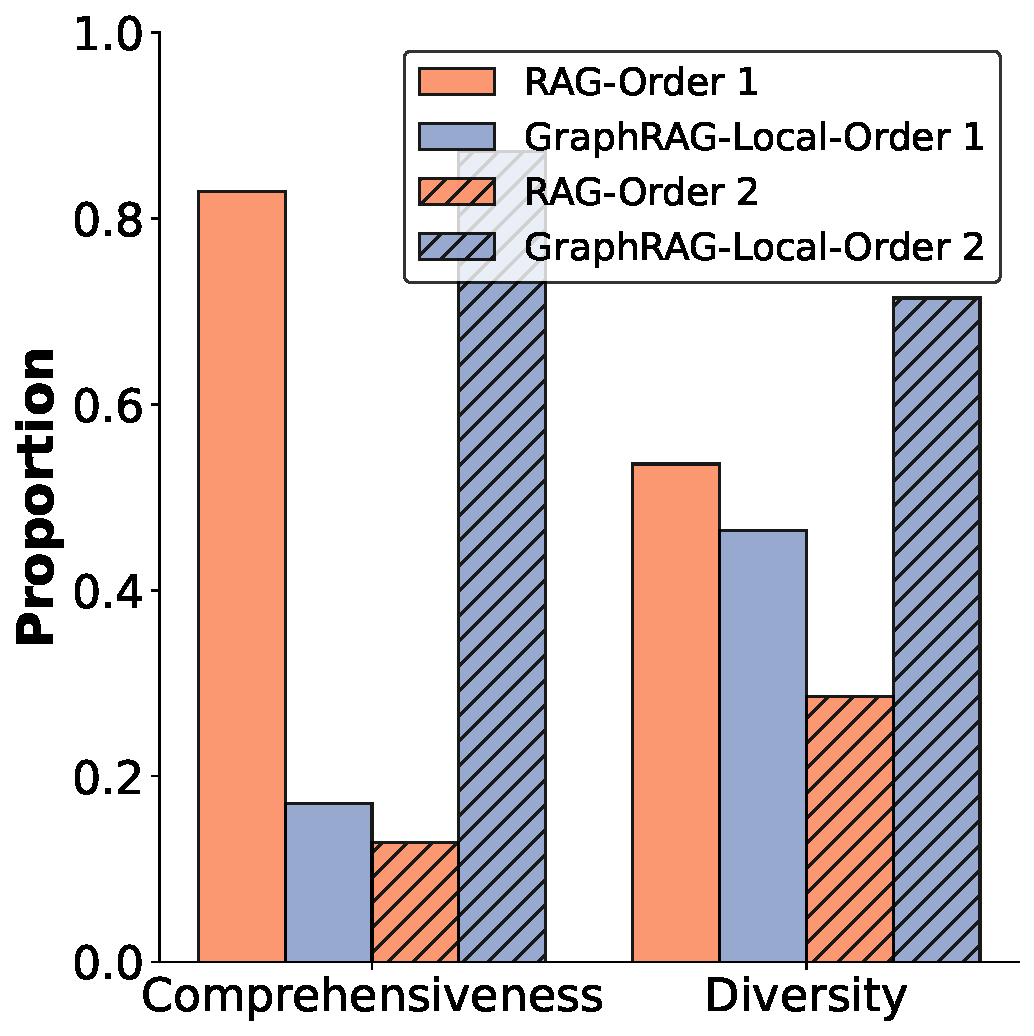
\includegraphics[width=\textwidth]{figures/QM_Local.pdf}
        \caption{QMSum Local}
        \label{fig:qmsum_local}
    \end{subfigure}
    \hfill
    \begin{subfigure}[b]{0.24\textwidth}
        \centering
        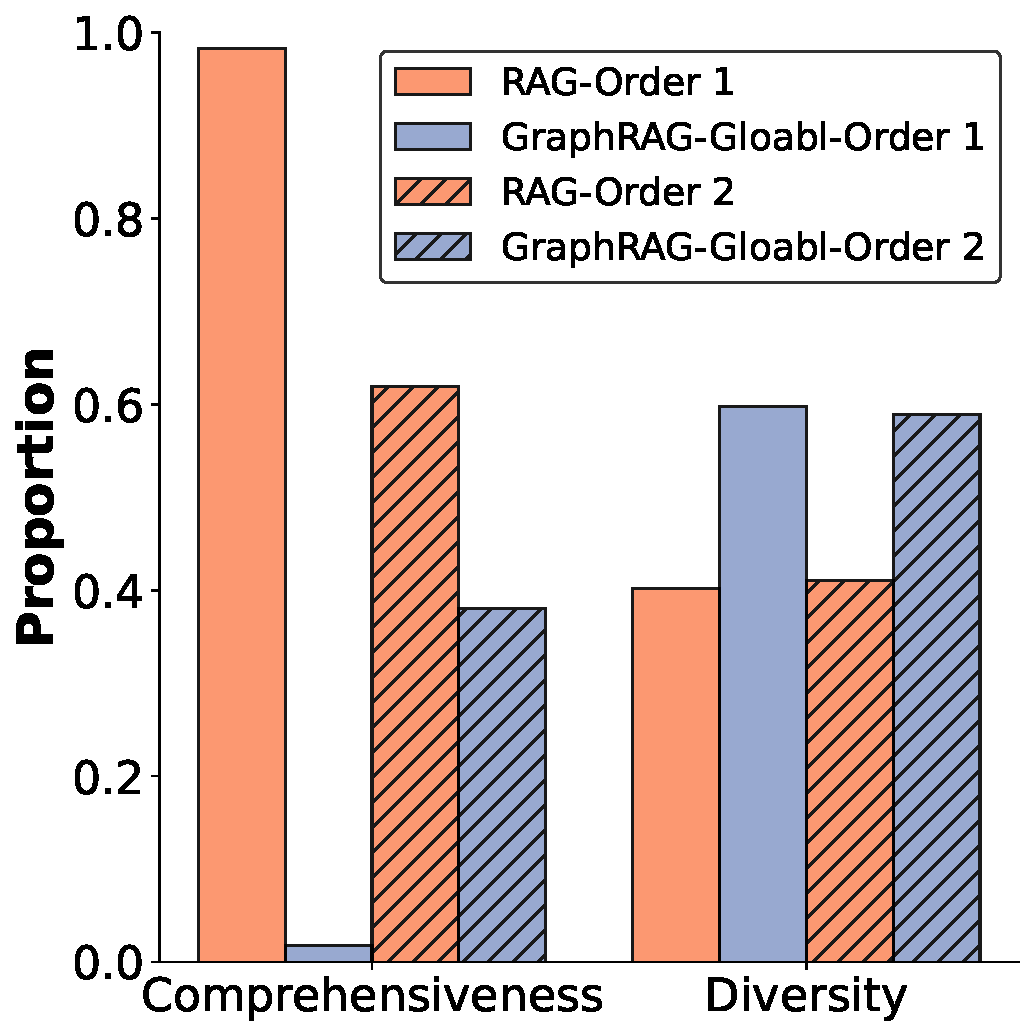
\includegraphics[width=\textwidth]{figures/QM_Global.pdf}
        \caption{QMSum Global}
        \label{fig:qmsum_global}
    \end{subfigure}
    \hfill
    \begin{subfigure}[b]{0.24\textwidth}
        \centering
        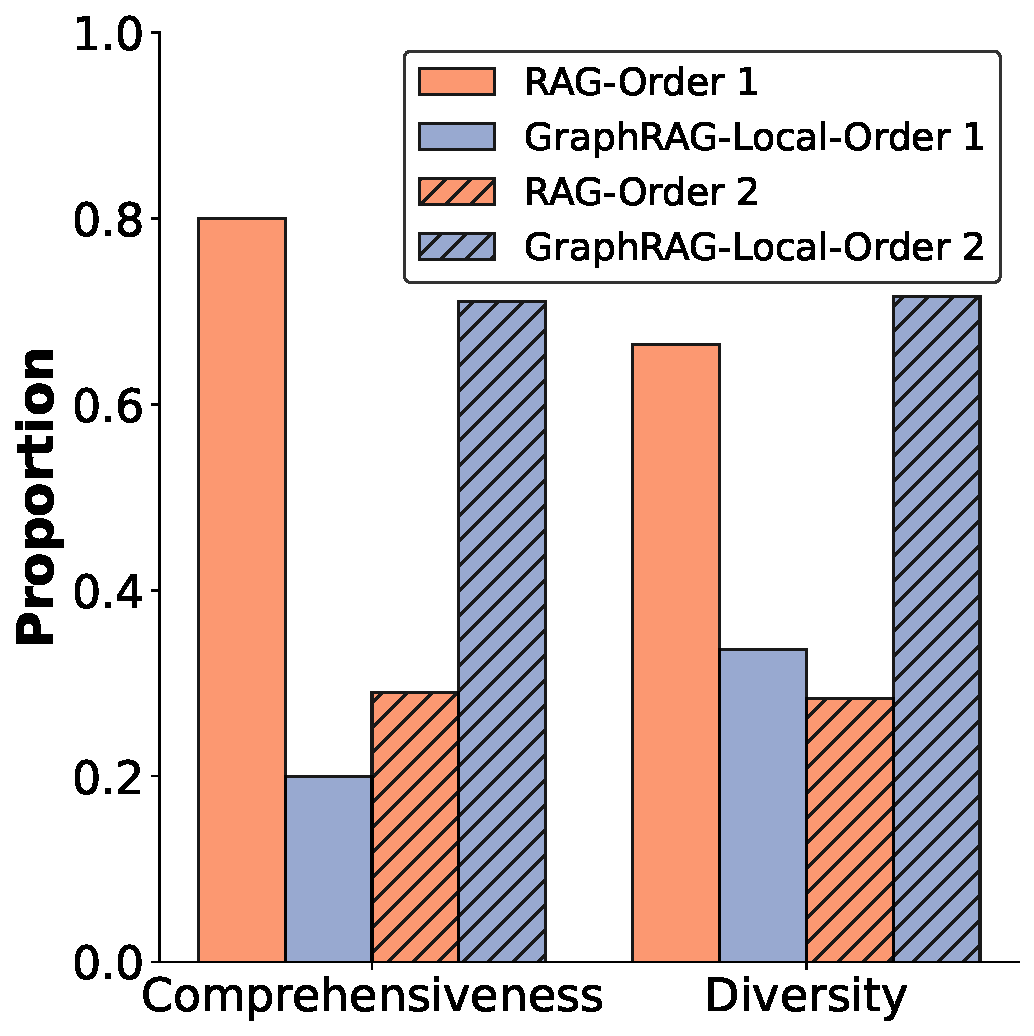
\includegraphics[width=\textwidth]{figures/Story_Local.pdf}
        \caption{ODSum-story Local}
        \label{fig:odsum_local}
    \end{subfigure}
    \hfill
    \begin{subfigure}[b]{0.24\textwidth}
        \centering
        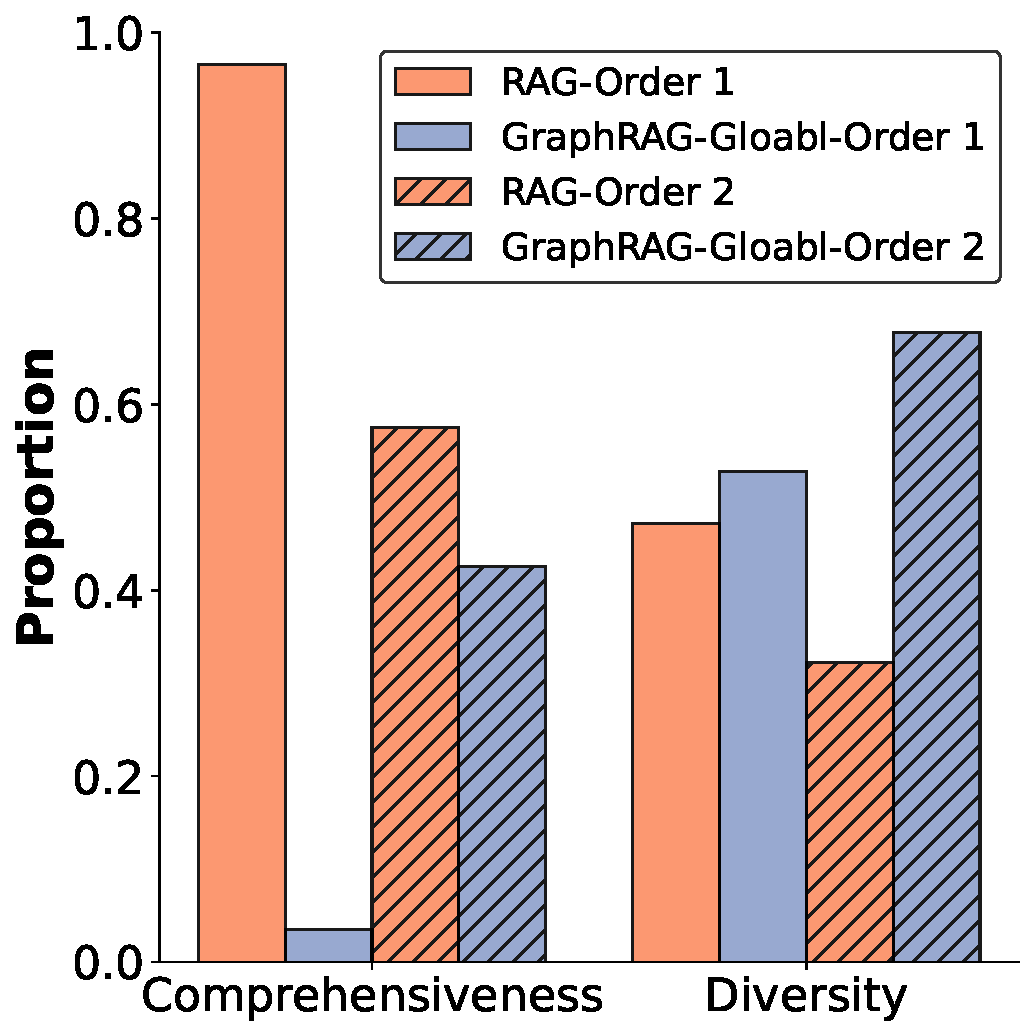
\includegraphics[width=\textwidth]{figures/Story_Global.pdf}
        \caption{ODSum-story Global}
        \label{fig:odsum_global}
    \end{subfigure}
    \vspace{-0.1in}
    \caption{Comparison of LLM-as-a-Judge evaluations for RAG and GraphRAG. "Local" refers to the evaluation of RAG vs. GraphRAG-Local, while "Global" refers to RAG vs. GraphRAG-Global. }
    \label{fig:summ_comparision}
    \vspace{-0.15in}
\end{figure*}

% \vspace{-0.05in}
\subsection{Summarization Experimental Results}
% \vspace{-0.05in}
\label{sec:summ_result}

We evaluate on vanilla RAG and GraphRAG methods, along with the Integration strategy discussed in Section~\ref{sec:improve_qa}. 
The results of Llama3.1-8B model on Query-based single document summarization and multiple document summarization are shown in Table~\ref{tab:summ_single} and Table~\ref{tab:summ_multi}, respectively. The results of Llama3.1-70B are shown in Appendix~\ref{app:summ_result}. Based on these results, we can make the following observations: 
% \vspace{-0.1in}
\begin{enumerate}[leftmargin=*, itemsep=0pt, parsep=-1pt]
    \item {\bf RAG, RaptorRAG, and HippoRAG2 generally performs well on query-based summarization tasks}, primarily because they retrieve original text chunks that are more closely aligned with ground truth.
    \item {\bf KG-based GraphRAG benefit from combining triplets with their corresponding text}. This improves performance by incorporating more details, making predictions closer to the human-written ground truth summaries.
    \item {\bf Community-based GraphRAG performs better with the Local search method}. Local search retrieves entities, relations, and low-level communities, while the Global search method retrieves only high-level summaries. This demonstrates the importance of detailed information in the selected datasets.
    \item {\bf The Integration strategy often performs comparably to RAG alone}, suggesting that simply concatenating RAG and GraphRAG evidence does not reliably improve alignment with detailed ground-truth summaries.
\end{enumerate}



\subsection{Position Bias in Existing Evaluation}
\label{sec:summ_analysis}
Based on the results in Section~\ref{sec:summ_result}, Community-based GraphRAG, particularly with global search, generally underperforms RAG on the selected datasets. This observation contrasts with the findings of \citet{edge2024local}, where Community-based GraphRAG with global search outperformed both local search and RAG.

This discrepancy can be attributed to two key differences between our evaluation and that of \citet{edge2024local}. First, their study focuses on global summarization, which aims to capture high-level information from an entire corpus, whereas the datasets used in our evaluation involve queries targeting specific roles or events. Second, \citet{edge2024local} evaluate performance using LLM-as-a-Judge without ground-truth references, while we evaluate generated summaries against human-written references using ROUGE and BERTScore. These reference-based metrics emphasize factual coverage and fine-grained details, which may favor different retrieval behaviors.

To further investigate this difference, we follow \citet{edge2024local} and evaluate RAG and GraphRAG using LLM-as-a-Judge from two perspectives: \emph{Comprehensiveness} and \emph{Diversity}. Comprehensiveness measures how well a summary covers the details required by the query, while Diversity assesses whether the summary provides a broad and globally inclusive view. Prompt details are provided in Appendix~\ref{app:llmjudge_prompt}. For each query, we present summaries generated by RAG and GraphRAG to the LLM and ask it to select the better one under each criterion.

To examine potential position effects in LLM-as-a-Judge evaluations, we consider two presentation orders: Order~1 (O1), where the RAG summary appears first, and Order~2 (O2), where the GraphRAG summary appears first. For each setting, we report the proportion of times each method is preferred by the LLM, where a higher proportion indicates stronger performance under the given presentation order.
Figure~\ref{fig:summ_comparision} presents results comparing RAG with GraphRAG (Local) and GraphRAG (Global) on the QMSum and ODSum-story datasets; additional results are included in Appendix~\ref{app:llmjudge_result}. We make two key observations. 
First, \textbf{position bias~\cite{shi2024judging, wang2024eliminating} is clearly present in LLM-as-a-Judge evaluations for summarization}, as reversing the order of presented summaries leads to substantially different, and in some cases opposite, judgments. This effect is especially pronounced for the comparison between RAG and GraphRAG (Local), as shown in Figures~\ref{fig:qmsum_local} and~\ref{fig:odsum_local}. 
Second, in comparisons between RAG and GraphRAG (Global), RAG is consistently preferred in terms of Comprehensiveness, while GraphRAG (Global) is favored for Diversity (Figures~\ref{fig:qmsum_global} and~\ref{fig:odsum_global}). This suggests that \textbf{Community-based GraphRAG with global search emphasizes corpus-level coverage, whereas RAG is more effective at capturing fine-grained, query-specific details}.

Finally, we report additional summarization results with reranking and iterative retrieval in Appendix~\ref{app:sec:iterative_retrieval} and ~\ref{app:sec:reranking}. We also provide a detailed analysis of indexing time, retrieval latency, generation cost, and token and storage usage for both methods in Appendix~\ref{app:sec:time}. Furthermore, we examine graph construction with different LLMs for summarization tasks in Appendix~\ref{app:graphconstruction}.



\noindent\textbf{Summary.}
Across query-based summarization benchmarks, RAG and GraphRAG exhibit different generation characteristic. Under reference-based metrics, RAG typically better matches detailed, query-specific ground-truth summaries, whereas GraphRAG, especially community-based global retrieval, tends to produce more corpus-level and diverse summaries that can deviate from fine-grained details. We also find that LLM-as-a-Judge evaluation can be sensitive to presentation order, raising reliability concerns for judge-based comparisons. Overall, these results highlight the need to balance detail fidelity, diversity, evaluation reliability, and system cost when applying (Graph)RAG to query-based summarization.


